\chapter{Usecase}
\label{ch:usecase}
F: Um welches System geht es?

\cref{fig:foto_tureschliessanlage} zeigt eine Türschließanlage wie sie aktuell in Zügen der Intercity-Klasse von der Deutschen Bahn eingesetzt werden. Die Anlage wird durch einen pneumatischen Kolben angetrieben. Über eine Zahnstange treibt der Kolben ein Rad an, welches wiederum einen Bautenzug betätigt. Am einem Stahlseil, das über Umlenkrollen geführt wird, wird die Tür auf- bzw. zugezogen.

\todo{Beschriftungen in Foto einfügen. ggf als Positionsnummern}
\begin{figure}[ht]
	\centering
	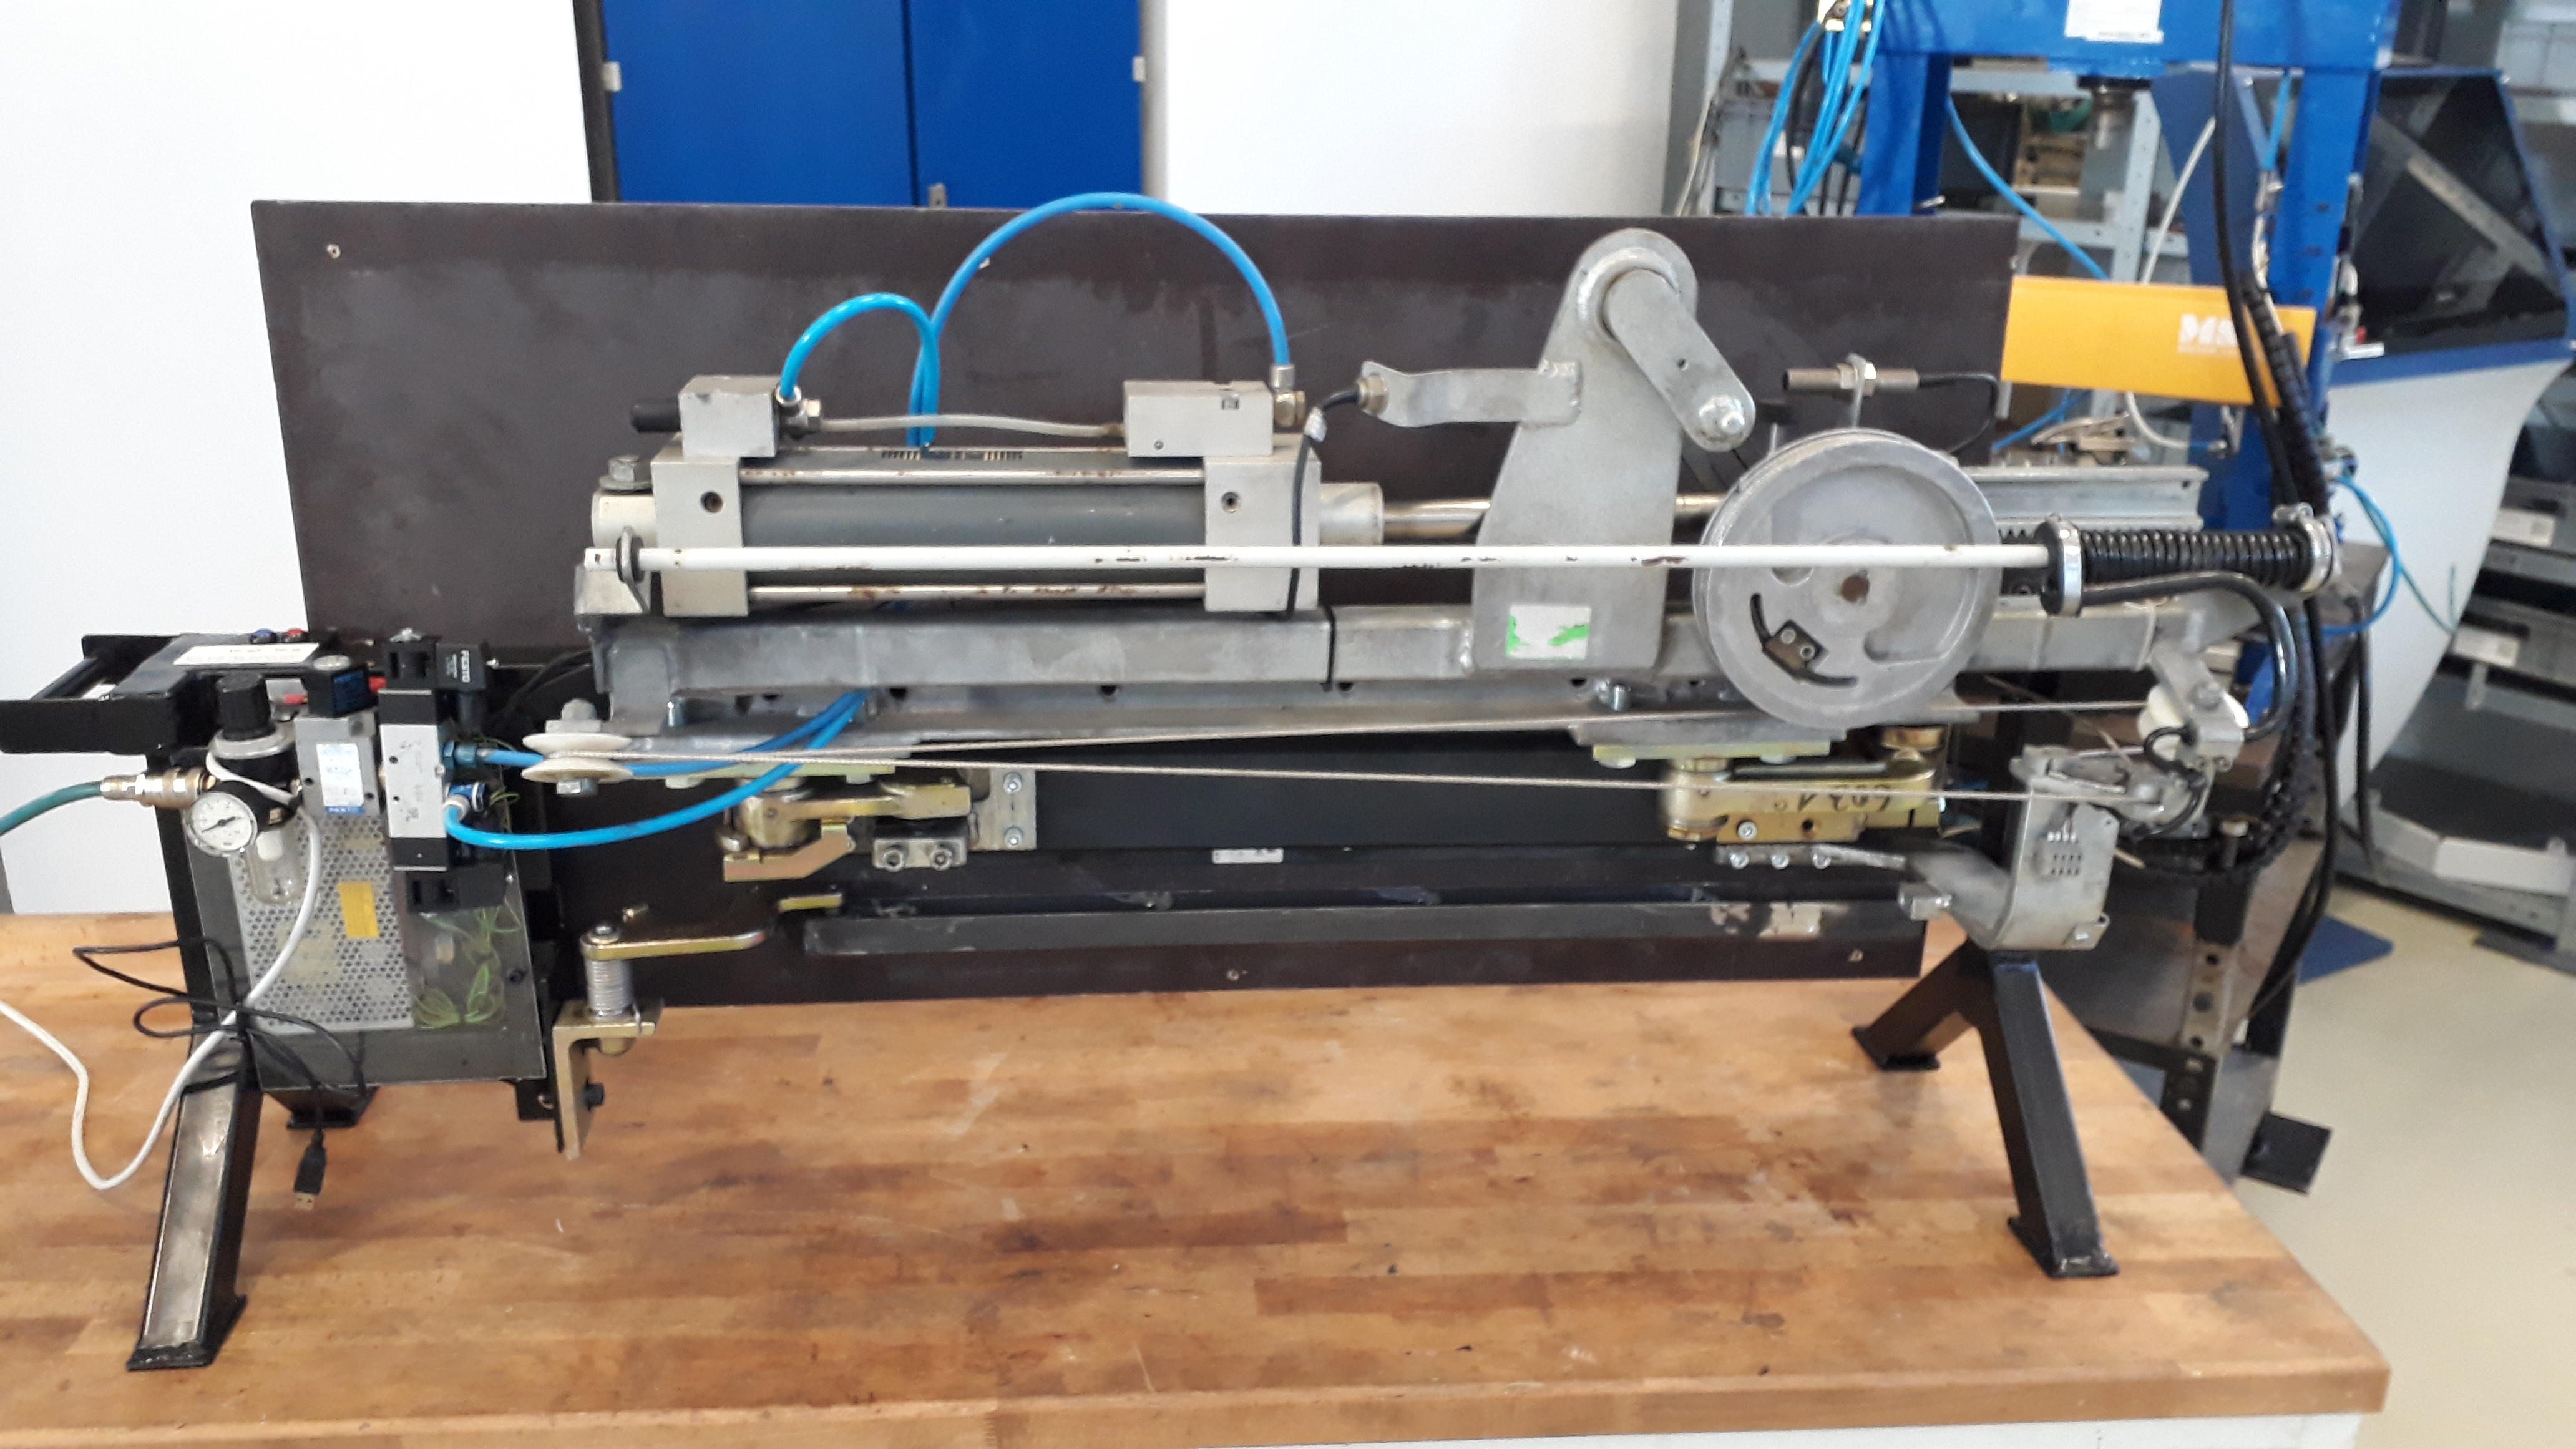
\includegraphics[scale=0.8]{Foto_Türschließanlage.jpg}
	\caption{Ausgebaute Türschließanlage eines Zuges der Intercity-Klasse (Deutsche Bahn)}
	\label{fig:foto_tureschliessanlage}
\end{figure}

F: wie wird die Anlage bisher gewartet

Wartungen der Anlage werden im Rahmen einer präventiven Instandhaltung durchgeführt. Zu diesem Zweck werden auch die Umlenkrollen regelmäßig ausgetauscht. Die Instandhaltungsmaßnahme wird entweder nach sechs Jahren oder nach \num{1.2} Millionen gefahrenen Kilometern durchgeführt~\cite{db.27.01.2021}.

F: warum müssen die Rollen gewechselt werden

Die Umlenkrollen aus Kunststoff \todo{CAD bild von rolle einfügen} sind ohne Wälzlager auf Bolzen montiert. Verschleiß und Materialermüdung sind in erster Linie an der Mantelfläche der Bohrung zu erwarten, an der die Rolle auf dem Bolzen aufliegt. Fortschreitende Rissbildung aufgrund von Materialermüdung bestimmt die Lebensdauer der Umlenkrollen. Mit steigendem Grad der Beschädigung steigt auch das Risiko eines Gewaltbruchs durch Überlast. In diesem Fall fällt die Türschließanlage aus und eine nicht planmäßige Instandsetzungsmaßnahme ist erforderlich.

F: welche Änderung der INSTANDHALTUNG ist denkbar?

Kann zu einem beliebigen Zeitpunkt der Zustand der Umlenkrollen bestimmt werden, so kann jederzeit der Bedarf einer Instandhaltungsmaßnahme eingeschätzt werden. Unerwartete Ausfällen können so vermieden werden (vgl. \cref{ch:instandhaltungsstrategien}). 

F: wie soll der usecase UMGESETZT werden

Die Instandhaltung der Umlenkrollen kann durch einem PdM-Ansatz gelöst werden. Voraussetzung dafür ist Erstens, dass Messwerte vorliegen, die Informationen über den Zustand der Umlenkrolle beinhalten. Zweitens sind diese Informationen in ein Entscheidungsmodel zu integrieren, das anhand von neuen Messwerten den Zustand der Rollen bestimmen kann. Drittens muss eine Infrastruktur geschaffen werden mit der in festgelegten Zeitabständen aktuelle Messwerte aufgenommen und verarbeitet werden können.
%===============================================================================
\section{Erfolgskriterien}
\label{sec:erfolgskriterien_usecase}
F: wieso müssen Erfolgskriterien definiert werden?

Um bestimmen zu können ob die Umstellung der Instandhaltung auf einen PdM-Ansatz sinnvoll ist, muss eine ausgiebige Nutzwertanalyse abgeschlossen und mit dem aktuell verwendetem PM-Ansatz verglichen werden. 

F: was ist das Problem bei der vergleichsführung?

Aufgrund der prinzipiell verschiedenen Natur von PM und PdM, lassen sich nur wenige Vergleichende kriterien bestimmen. Beispielsweise kann die Anzahl richtig positiver Vorhersagen -- also die Anzahl vermeidbarer Ausfälle -- nicht verglichen werden, weil bei einem PM-Ansatz dazu keine Informationen zur Verfügung stehen. Auch werden bei PM per Definition keine unnötigen Inspektionen durchgeführt, wie es bei PdM für falsch positive Meldungen der Fall wäre. Um einen Vergleich der beiden Ansätze erheben zu können, sind also allgemeinere vergleichende Kriterien zu finden.

Im Rahmen dieser Arbeit wird ausschließlich auf Kriterien eingegangen, die den Nutzwert des vorgeschlagenen PdM-Ansatzes quantifizieren. Die Kriterien werden für die Bewertung der maschinellen Lernmodelle herangezogen, die in \cref{sec:modelierung} erstellt werden. Die Beurteilung des besten Models ist die Grundlage auf der eine Kosten-Nutzen-Analyse durchgeführt werden kann. Die folgenden Kriterien definieren den Nutzen der PdM-Anwendung.

\textbf{Komplexität}

Idealerweise soll das Modell nicht nur möglichst korrekte Vorhersagen über den Zustand der Umlenkrollen abgeben können, sondern auch Informationen extrahieren, die für Verbesserungen der Konstruktion verwendet werden können. Dafür ist ein Model nötig dessen Entscheidungverfahren nachvollziehbar ist. Ein zu komplexes Model kann nicht unter praktikablen Bedingungen ausgewertet werden. Aus diesem Grund ist ein einfach nachzuvollziehendes Model einem komplexeren vorzuziehen.

\textbf{Qualität der Vorhersagen}

Damit der Usecase einen Mehrwert gegenüber dem vorherigen Vorgehen bietet, müssen die Vorhersagen des Models ein Mindestmaß an Genauigkeit bieten können. Die Zahl falsch positiver, wie auch falsch negativer Vorhersagen (Fehlalarme bzw. unentdeckte Beschädigungen), sollten möglichst gering ausfallen. Ein Mindestmaß für beide Eigenschaften hängt von der Qualität des gegenüber stehenden PM-Usecases ab. Weil -- wie einleitend erwähnt -- dieses Kriterium keinen direkten Vergleich zwischen dem PM- und PdM-Ansatz zulässt, werden Annahmen für die Mindestmaße getroffen (s. \cref{sec:praeferenzfunktion}).

Bei Qualität der Vorhersagen sind falsch positive Vorhersagen geringer zu wichten als falsch negative. Falsch positive Vorhersagen haben eine unnötige Inspektion oder Austausch der Komponente zufolge, wohingegen falsch negative Vorhersagen zu einem unerwarteten Ausfall führen. Im ersten Fall entstehen Kosten durch Verschwendung; im zweiten durch die notwendige Behebung einer Störung. Letzteres ist jedoch in der Regel mit höheren Kosten verbunden. Deswegen wird falsch negativen Vorhersagen ein höheres Gewicht zugeschrieben als falsch positiven Vorhersagen \todo{Verweis auf Paarvergleich einfügen}. 
Das Kriterium lässt sich in Form der Sensitivität und Relevanz direkt auf die Bewertung des verwendeten Vorhersagemodelle anwenden.
%===============================================================================
\section{Einordnung in den Kontext der Bahntechnik}
\label{sec:kontext_bahntechnik_von_usecase}
Der eröffnete Usecase beruht auf allgemeinen Prinzipien von PdM. Darüberhinaus gehend ist es sinnvoll den Usecase in den Kontext der praktischen Bahntechnik ein zu ordnen. Insbesondere eine Diskusion über den tatsächlichen Bedarf, als auch eine Darstellungen des angewandten Wartungsvorgehen ist für eine Bewertung des Usecases zuträglich.

Um den Usecase in den Kontext der Bahntechnik zu stellen, wurden zwei Interviews mit Sachverständigen der Deutschen Bahn und der Hochbahn Hamburg geführt. Die folgenden Abschnitte geben die wichtigsten Ergebnisse dieser Interviews wieder.
%===============================================================================
\subsection{Interview: Hochbahn Hamburg}
\label{subsec:interview_hochbahn}
\textit{Interview mit Jürgen Beck~\cite{hochbahn.23.11.2020} am {23.11.2020}}

Herr Beck benannte im Allgemeinen Lager als Komponenten, deren Wartungen von Kenntnissen über den aktuellen Zustand profitieren kann. Sie gehören zu den Komponenten, die dem größten Verschleiß unterworfen sind und daher häufig zu ersetzen sind. Die Umlenkrollen sind nicht in Verbindung mit einem Wälzlager montiert, sondern stützen sich direkt an deren Aufhängung ab. Verschleiß -- bedingt durch Relativbewegung zwischen Bolzen und Rolle -- tritt also an der Umlenkrolle selbst auf. Vor diesem Hintergrund ist die Wahl, die Umlenkrollen mit einem PdM-Ansatz instand zu halten, ebenso sinnvoll wie für Wälzlager.

Bezogen auf den Betrieb der Hochbahn in Hamburg wurde diskutiert welche Auswirkungen ein Ausfall der Türschließanlage hat und ob sich daraus ein Bedarf für den vorgeschlagenen Usecase ableiten lässt. Herr Beck betonte, dass eine Störung der Türanlage nur in Ausnahmefällen einen bedeutsamen Einfluss auf den Betriebsablauf hat. Für einen solchen Ausnahmefall müssten mehrere Türschließanlage an dem selben Waggon ausfallen und der Waggon dürfte nicht durch Zwischentüren mit den anhängenden Waggons verbunden sein. In einem solchen Fall ist ein sicherer Betrieb des Waggons nicht mehr möglich, weil Fluchtmöglichkeiten unzulässig beschränkt sind. Es wird nicht erwartet, dass eine derartiger Ausnahmefall eine Umstellung der Instandhaltung auf einen PdM-Ansatz rechtfertigen kann. Dies ist der auch der Grund dafür warum die Hochbahn Hamburg aktuell nicht an der Umsetzung einer PdM-Anwendung arbeitet, wie sie zu Beginn dieses Kapitels vorgeschlagen wurde.
%===============================================================================
\subsection{Interview: Deutsche Bahn}
\label{subsec:interview_deutsche_bahn}
\textit{Interview mit Dr. Jörg Lehmann~\cite{db.27.01.2021} am {27.01.2021}}

Herr Lehmann schrieb die das Vorgehen bei der Instandhaltung von Reginonal- und Fernverkehrszügen wie folgt:\\
Unterschieden wird zwischen der \textit{betriebsnahen} und der \textit{schweren} Instandhaltung. Die betriebsnahe Instandhaltung wird durch den Zugbetreiber durchgeführt und umfasst Instandhaltungsmaßnahmen, die die kurzfristige Verfügbarkeit des Zuges gewährleisten. Im Gegensatz zur schweren Instandhaltung wird sie nach Bedarf durchgeführt. Neben Reinigungsarbeiten und Reparaturen an Interiör, umfasst sie auch Arbeiten an technischen Systemen des Zuges. Eine Türstörung kann laut Lehmann in der Regel im Rahmen einer betriebsnahen Instandhaltung behoben werden. Das bedeutet, dass Maßnahmen zur vorausschauenden Instandhaltung kurzfristig umgesetzt werden können, ohne dafür neue Strukturen schaffen zu müssen.

Die schwere Instandhaltung wird entweder nach sechs Jahren Betriebsdauer oder nach \num{1.2} Millionen gefahrenen Kilometern vorgenommen. Sofern die festgelegte Kilometeranzahl noch nicht erreicht ist, kann nach einer Einschätzung durch Sachverständige, das Intervall	auf \num{8} Jahre angehoben werden. Zu Beginn der schweren Instandhaltung wird eine Eingangsuntersuchung vorgenommen. Daran schließen sich Instandhaltungsmaßnahmen in Form von Plan-, Sicherheits- und Außerplanarbeiten an. Planarbeiten stehen bereits im Vorfeld der schweren Instandhaltung fest und werden grundsätzlich durchgeführt. Außerplanarbeiten bedürfen einer nachträglichen Auftragsstellung. Die Auftragsstellungen erfolgen auf Basis der Ergebnisse der Eingangsuntersuchung. Gegeben dem Fall, dass durch die PdM-Anwendung Informationen über den Zustand der Umlenkrollen vorliegen, kann ihre Instandhaltung im Rahmen von Planarbeiten erledigt werden. Es wird also ein Zeitvorsprung gewonnen, der eine Planung ermöglicht.

Die Aussagen von Herrn Beck bezüglich des Bedarfs des Usecases teilt Herr Lehmann. Auch seiner Ansicht nach ist der Einfluss einer Türstörung auf den Betriebsablauf klein, weswegen wirtschaftlicher Mehrwert nicht zu erwarten sei.
%===============================================================================


